\chapter{Introducción Específica} % Main chapter title

\label{Chapter2}
%
%%----------------------------------------------------------------------------------------
%%	SECTION 1
%%----------------------------------------------------------------------------------------
%La idea de esta sección es presentar el tema de modo que cualquier persona que no conoce el tema pueda entender de qué se trata y por qué es importante realizar este trabajo y cuál es su impacto.
%\label{sec:ejemplo}
En este sección se detallaran las tareas que se realizaron, que contratiempos se tuvieron y cuales fueron los requerimientos.

\section{Objetivos y alcances}

\subsection*{Objetivos}
    Desarrollar un software que permiea controlar, monitorear y supervisar el proceso de fermentación del vino en las bodegas en forma automática. Aprovechando el proyecto CIAA, se utilizó esta plataforma ya que está preparada especialmente para aplicaciones industriales, siendo esta libre y gratuita.
\subsection*{Alcance}
  \begin{itemize}
      \item Sensar la temepratura de un tanque de fermentacion de ya se para vinos tintos o blancos.
      \item Controlar que la temperatura se mantenga dentro del rango correspondiente según el tipo de vino. 
      \item En caso de corte de energia se notificar vía SMS a un celuar de contacto.
      \item Mensajes de alerta vía SMS en caso de temperatura fuera de rango.
      \item Diseño de una página que permita mostrar la informacion del sistema y realizar las configuraciones necesarias.
      \item Diseño de una placa básica para mostrar el funcionamiento del sitema.
  \end{itemize}

  \section{Requerimientos}

Estos fueron consensuados con el responable de la Bodega Chico Zossi, para trabajar sobre un caso real. 

\begin{enumerate}[label*=\arabic*.]
  \item Medición de Temperatura:
    \begin{enumerate}[label*=\arabic*.]
      \item  Se requiere medir la temperatura de un tanques.
      \item La resolución de debe ser de $\pm 1^oC$.
    \end{enumerate}
  \item Comunicación:
    \begin{enumerate}[label*=\arabic*.]
      \item Debe poder transmitir mensajes SMS notificando el estado/cambios producidos.
      \item Acceso web para la configuración de los parámetros requeridos de temperatura. 
    \end{enumerate}
  \item Funcionamiento del Sistema embebido:
    \begin{enumerate}[label*=\arabic*.]
      \item El sistema deberá mantener la temperatura controlada a los parámetros configurados por el usuario. Para ello deberá hacer uso del actuadores.
      \item Deberá alertar si hay corte de energía mediante un SMS.
      \item Deberá mostrar el nivel de batería.
  \end{enumerate}
\end{enumerate}


\section{Desglose de tareas - GANTT}
Para llevar el proyecto a cabo se desarrolló la siguiente planificación de tareas y se estimaron que tiempos debían emplearse para cada una de ellas.

Se analizaron que tareas debian realizarse primero y cuales eran sus dependencias. De esta forma, si se presentara alguna complicación poder tener un análisis más completo de cómo afectaría a la fecha de entrega del proyecto.

Todo este estudio fue aprovechado de haber de lo aprendido en la asignatura de Gestion de Proyectos. Se puede ver en la figura \ref{fig:gantt} el plan de trabajo.

\begin{landscape}
  \pagestyle{empty}
  \begin{figure}[htb]
      \centering
      %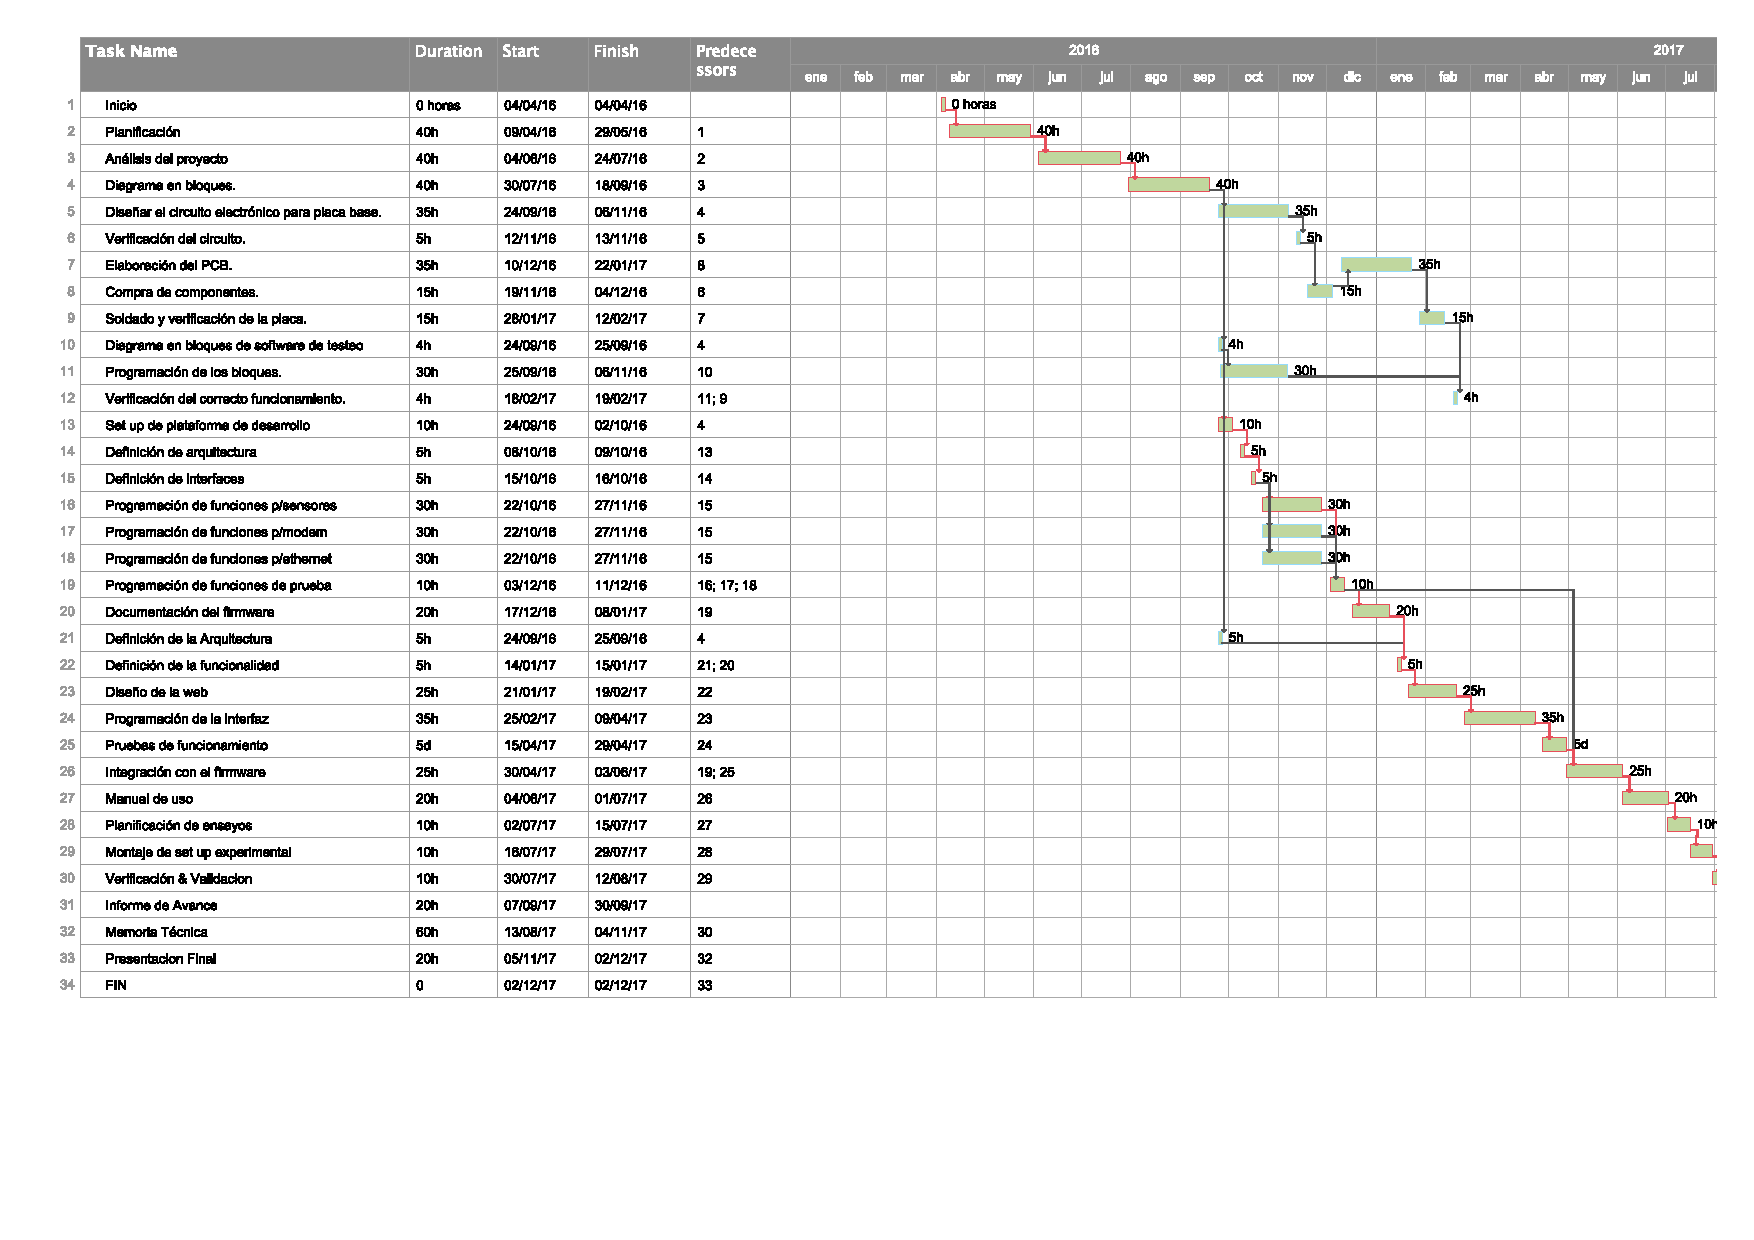
\includegraphics[page=1,clip, trim=0.5cm 4cm 16.3cm 0cm, width=1.00\textwidth]{./Figures/task_list.pdf}
          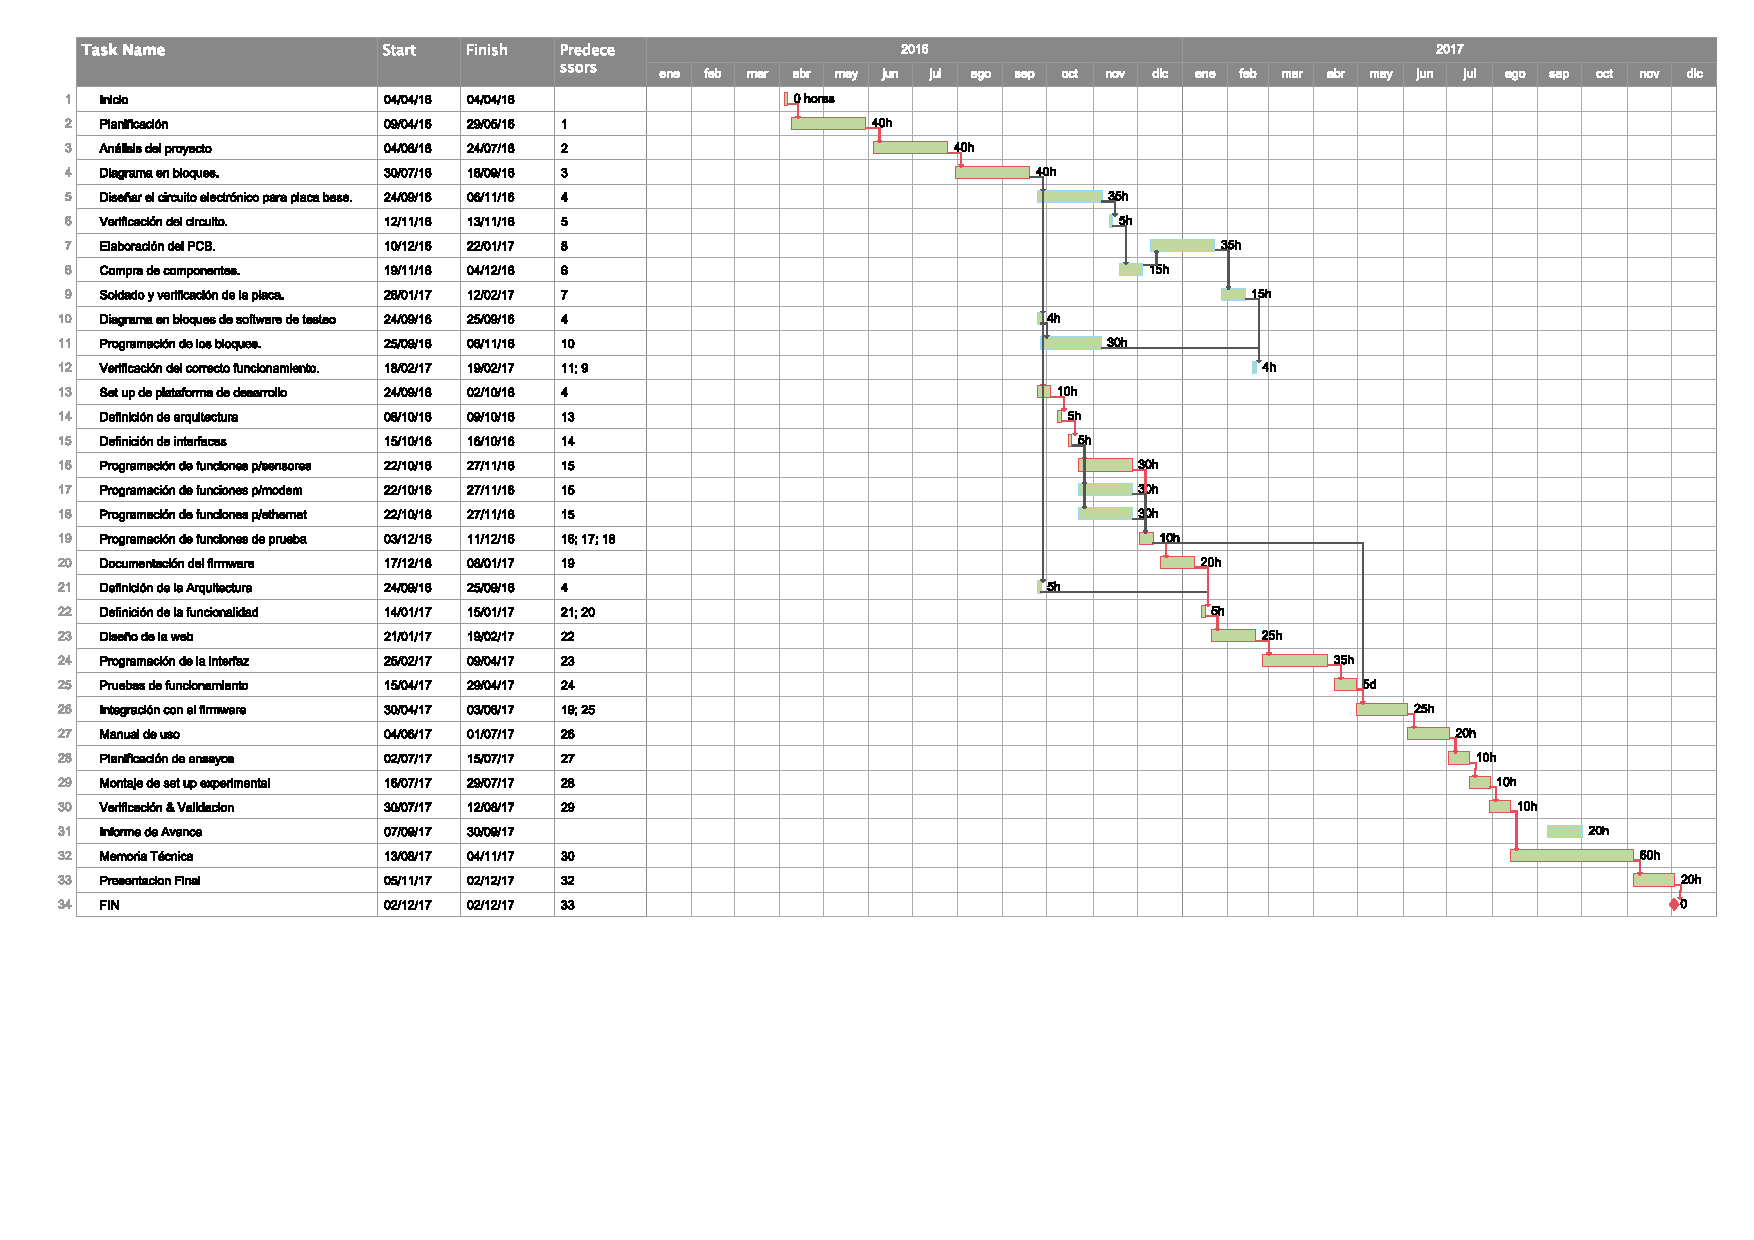
\includegraphics[page=1,clip, trim=0.5cm 5cm 0cm 0cm, width=1.70\textwidth]{./Figures/gantt.pdf}
      \caption{Listado de tareas, y plafinicación de tiempos de la implementación.}
      \label{fig:gantt}
  \end{figure}
\end{landscape}


Dada a la falta de experiencia en determinados temas, se requirió más tiempo de lo planificado.  En la tabla \ref{tab:update_task}, se aprecia el tiempo real y cuales fueron las tareas que requirieron más tiempo.

\begin{table}[hp]
  \begin{tabular}{|c|c|c|c|c|}
    \hline
       &       & \multicolumn{2}{c|}{ Tiempo} & \%  \\ \cline{3-4}
    Nro& Tarea &  Estimado &  Real & a más \\
    \hline
    9 & Soldado y verificación de la placa & 15h & 24 & 60 \\
    18 & Programación de funciones p/ethernet & 30h & 50h & 66,7 \\
    23 & Diseño de la web & 25h & 35h & 40 \\
    \hline \hline
  \end{tabular}
  \caption{Comparación del tiempo planificado con el real.}
  \label{tab:update_task}
\end{table}

Con lo cual hay una diferencia de 39 horas a más de lo planificado. Siendo que para el desarrollo de todo el proyecto se habían estimado 617 horas podemos concluir que la estimación de los tiempos no estuvo mal. 
Dado que habían temas que no se conocían con profundiad y de haber sido crítica la fecha de entrega se hubiera buscando ayuda de otro programador para poder avanzar en forma paralela. 

